\documentclass[hyperref={pdfpagelabels=false}]{beamer} 

\usepackage[portrait]{sfocs-poster}
\usepackage{lipsum}
\usepackage{rotating}
\usebackgroundtemplate{%
	% image as background
		\tikz\node[opacity=0.9] {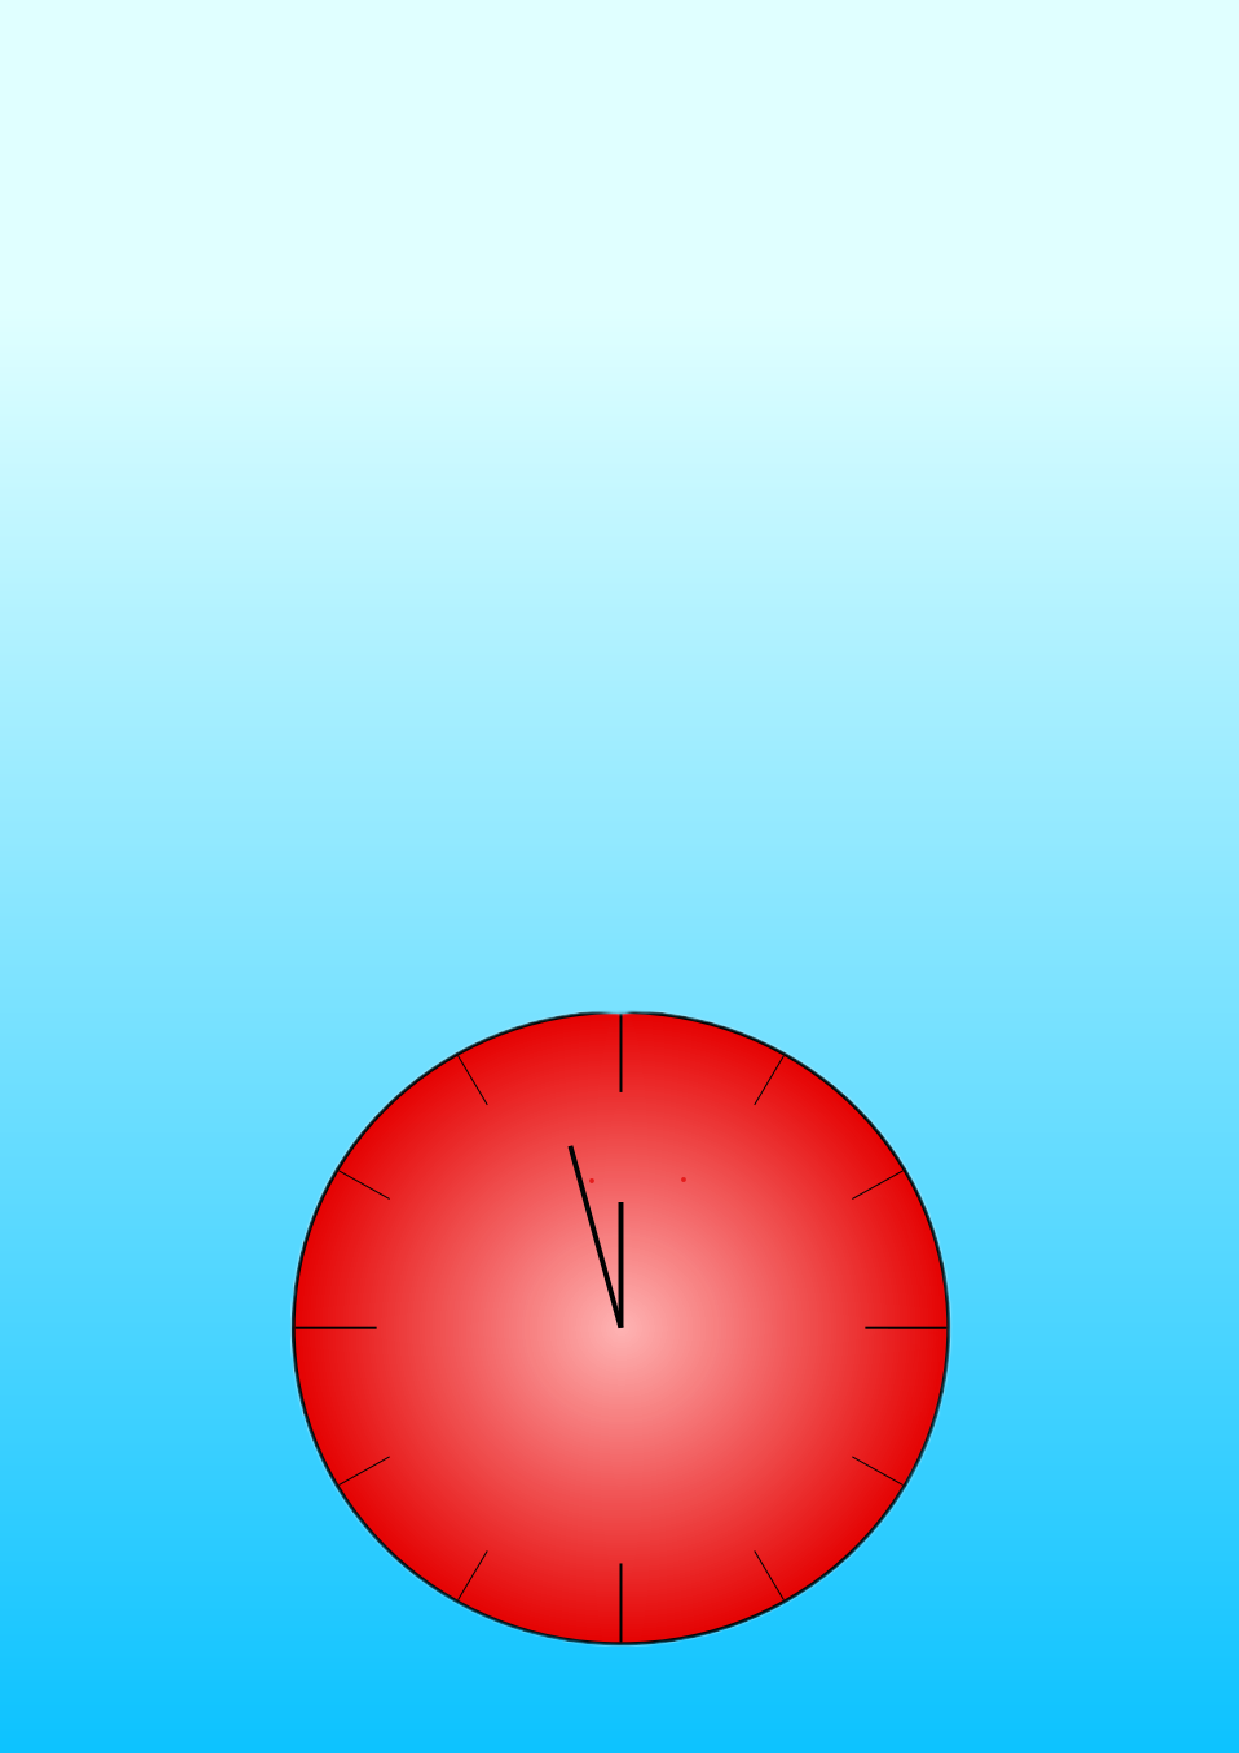
\includegraphics[height=\paperheight,width=\paperwidth]{img/pg}};
	% plain color 
	%\tikz[remember picture,overlay] \fill[game] (current page.north west) rectangle (current page.south east); 
}
%
% sample boxes 
% 
\tcbset{
        framedbox/.style={
					enhanced, fontupper=\large,left=.75cm,fonttitle=\LARGE,toptitle=.25cm,bottomtitle=.25cm,halign title=center
        },
}

\newtcolorbox{basebox}[3][]{framedbox,coltitle=#2,colback=#3,coltext=#2,title=#1,colframe=#3,sharp corners}
\newtcolorbox{baseroundedbox}[3][]{framedbox,colback=#3,colframe=#3,coltitle=#2,coltext=#2,title=#1,,rounded corners,arc=15pt}
\newtcolorbox{transparentbox}[4][]{framedbox, colback=#3,colbacktitle=#3,colframe=#3,coltitle=#2,coltext=#2,title=#1,frame style={color=#3},opacitybacktitle=#4,opacityback=#4,opacityframe=#4,opacityfill=#4}
\newtcolorbox{blankbox}{blanker,fontupper=\LARGE}


% draw a grid
%\beamertemplategridbackground[0cm]

\begin{document}

\begin{frame}

	\begin{textblock}{45}(2,1)
		\begin{blankbox}
			
\includegraphics[width=1000pt]{img/gamename.png} \\\hspace*{\fill} \\ \\
		\end{blankbox}
	\end{textblock}




\begin{textblock}{35}(1,42)
		\begin{blankbox}
		\huge \textbf{ Brief Instructions On The Game} \\

						\begin{itemize}
							\item Health Threat Drop: The dis-alarmed Health threat level
							\item Citizen Trust: The faith citizens in an area have in its governor
							\item External Safety: The safety guaranteed of the personnel and material inflow
							\item Disposable Money: The maximum financial aid offered to concerned institute
						\end{itemize}
			
		\end{blankbox}
	\end{textblock}





	\begin{textblock}{30}(28,92.5)
		\begin{blankbox}
			
\includegraphics[width=205pt]{img/Teamlogo.png}

		\end{blankbox}
	\end{textblock}

	\begin{textblock}{20}(71,3.8)
		\begin{blankbox}
			\Huge\textbf{MINIMALISM}

\vspace{0.4cm}

			\textbf{SIMPLICITY}
\vspace{0.4cm}

\textbf{ENTERTAINMENT}
		\end{blankbox}
	\end{textblock}
	\begin{textblock}{40}(58,16)
		\begin{blankbox}
\vspace {0.4cm}
Out of humanistic trans-regional assistance, the players, more often than not, are pressed to make moral decisions balncing the safety of districts by tranfering the CR (Critical Resources) lightning fast.Maintaining the regional CPs (Control Points) above 0 in certain durations leads to victory. Alternatively, any CPs hitting 0 would instantly indicate failure.\vspace {0.4cm}

 Terminator recreates for the players the scenario where countless medical workers, policy makers and all the other concerned parties had to make tough decisions facing extremelystressful situations just to save our lives and protect our countries as best as they can during the real pandemic COVID-19 last year. May their great spirit inspire us.\vspace {0.4cm}
			
		\end{blankbox}
	\end{textblock}



	% #1: box width 
	% #2 #3: coordinates on percent 


	
	\begin{textblock}{50}(25.5,70)
		% no title provided, extra parameter is opacity in [0,1] 		
		\begin{transparentbox}{black}{red}{.2}
				\centering \vspace{.25cm}
				\huge\textbf{Main Appeal}\vspace{1cm}

\begin{itemize}\itemsep .85cm
			\centering{ \item Highly Customized User Control

				\item Simple yet ingenious Operation

				\item Minimalist User Interface

				\item  Diverse Gaming Modes}
\end{itemize}       	 

		\end{transparentbox}
	\end{textblock} 

	% option [0,1] means box anchor is bottom left	
	\begin{textblock}{80}[0,1](1,100)
		\logos[light]
	\end{textblock}

	% option [1,1] means box anchor is bottom right	
	\begin{textblock}{30}[1,1](100,100)
		\begin{blankbox}
			\huge\textbf{{THREE TO ONE:}} \\
			\Large{Zining Wang (C)}\\ 
			Yifan Jia  \\
			Qiao Liu \\\hspace*{\fill} \\
			Our attention to the current affairs has inspired the game. Now you can be the protagonist and savior. Good Luck!
			
		\end{blankbox}
	\end{textblock}

	\begin{textblock}{10}(10,70)
		\begin{blankbox}
			\centering
			
\includegraphics[height=400pt]{img/ai97b-ej97b.png}
		\end{blankbox}
	\end{textblock}

	\begin{textblock}{10}(80,70)
		\begin{blankbox}
			\centering
			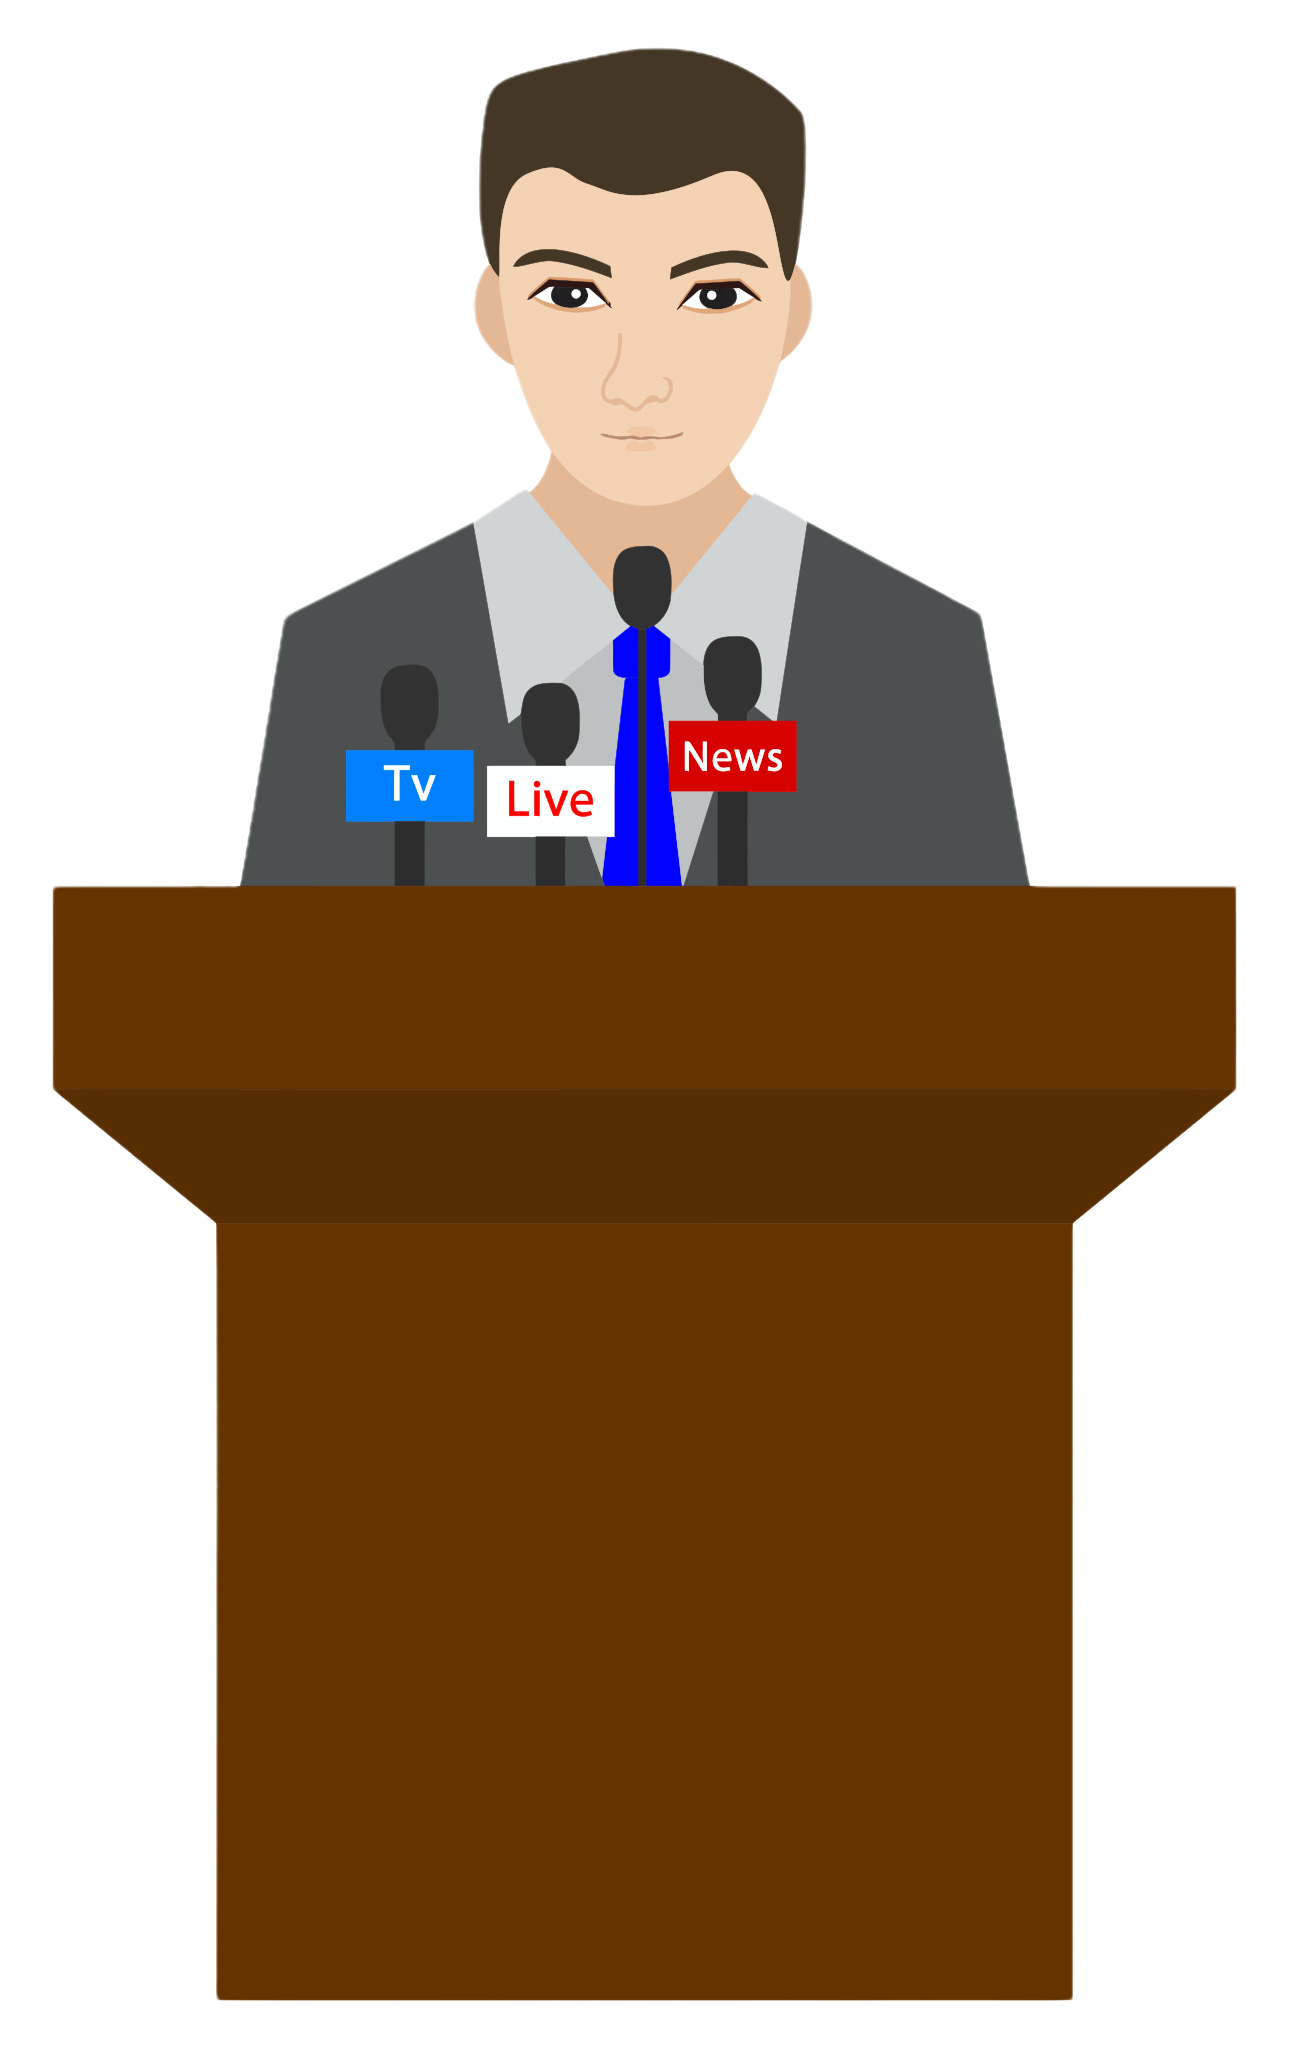
\includegraphics[height=400pt]{img/arn28-kj5eh.png}
		\end{blankbox}
	\end{textblock}

	\begin{textblock}{40}(38,42)
		\begin{blankbox}
			\centering
			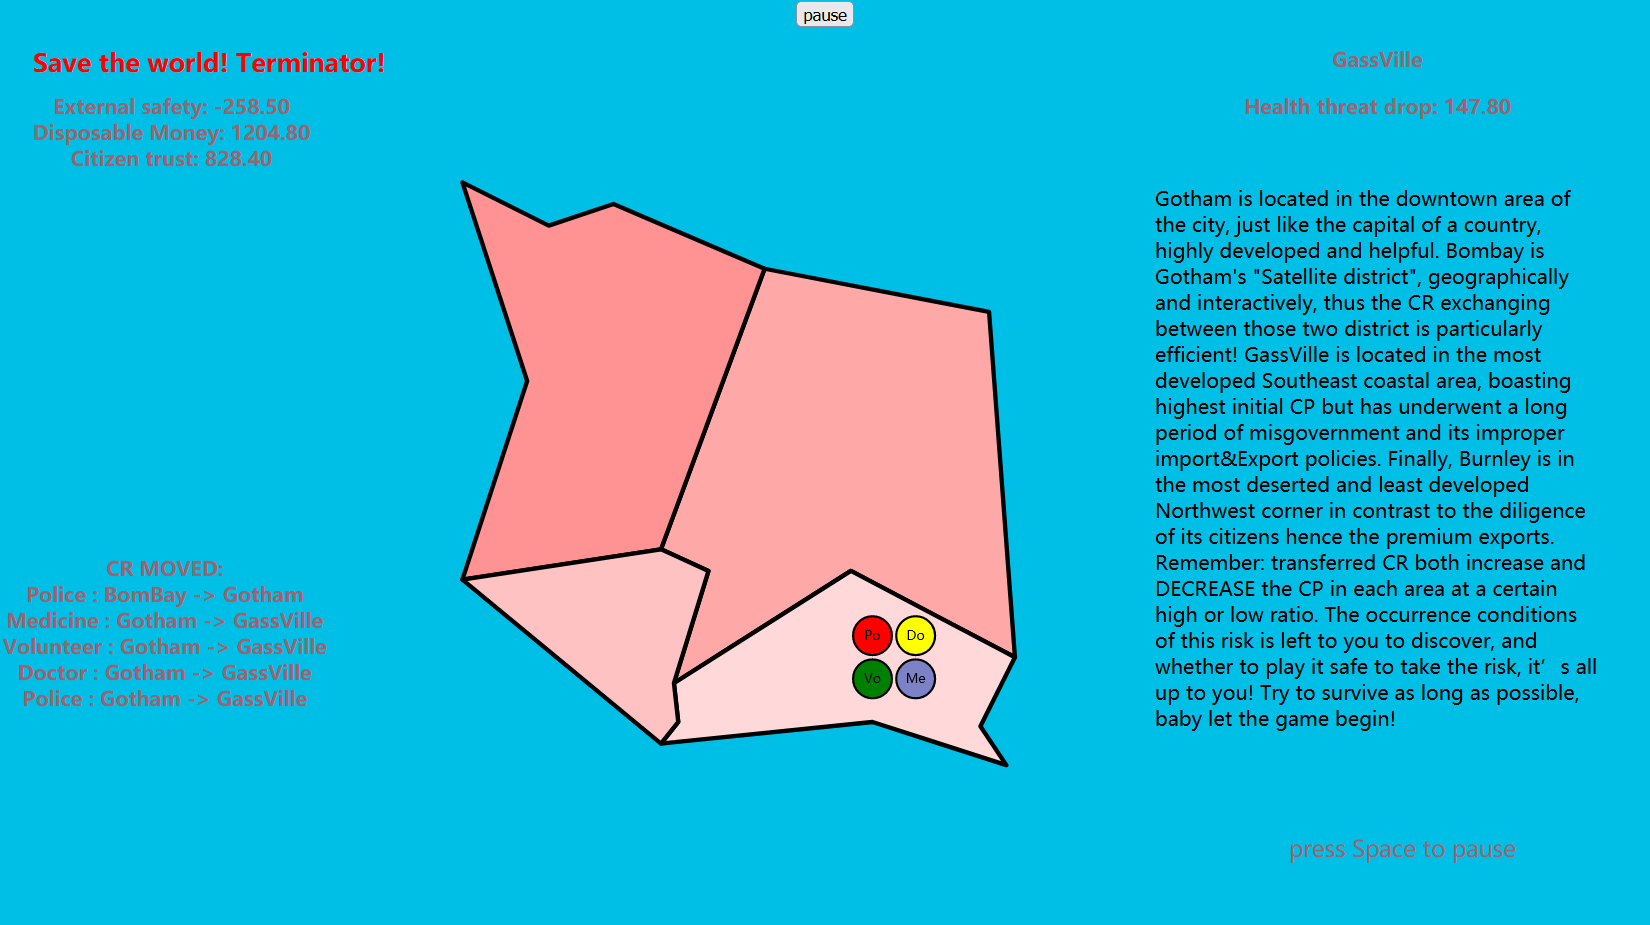
\includegraphics[ height=570pt]{img/newDemo}
		\end{blankbox}
	\end{textblock}
\begin{turn}{60}
	\begin{textblock}{1}(67,3)
		\begin{blankbox}
			\centering
			
\includegraphics[height=200pt]{img/aLine}
		\end{blankbox}
	\end{textblock}
\end{turn}


	\begin{textblock}{10}(1.3,13.3)
		\begin{blankbox}
			\centering
			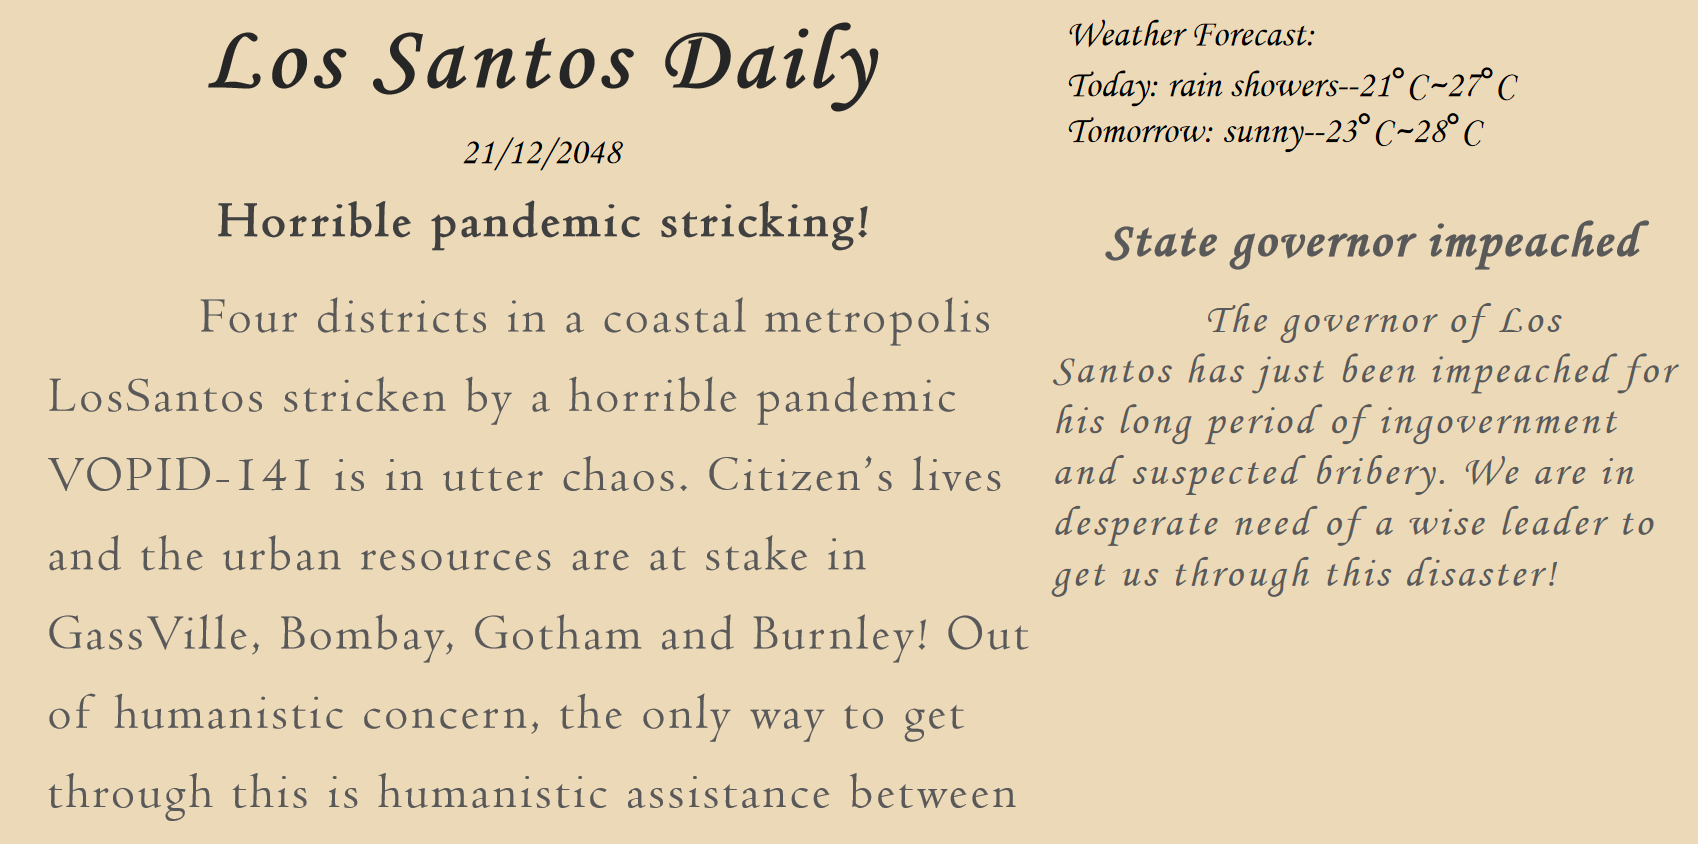
\includegraphics[angle=8,height=600pt]{img/news.png}
		\end{blankbox}
	\end{textblock}


\end{frame}

\end{document}

transparent box 
larger title font 
no gradient 
plain box
